% Documentation of the Perceptron Project
% Subject: Digitaldesign at the Ernst-Abbe-Hochschule Jena
% Author: Fabian Franz

% Packages and Modules
\documentclass{article}
\usepackage{array}
\usepackage{amsmath}
\usepackage{hyperref}
\usepackage{graphicx}
\usepackage{circuitikz}
\usepackage[english]{babel}
\usepackage[utf8]{inputenc}
\usepackage[a4paper, margin=1in]{geometry}
\usepackage{tikz}
\usepackage{float}
\usepackage{mathrsfs}
\usepackage[section]{placeins}

% Tikz config
\usetikzlibrary{calc}
\usetikzlibrary{positioning}

% Graphic config
\graphicspath{{./images/}}
\usetikzlibrary{shapes,arrows}
\numberwithin{equation}{section}

% Equation conditions
\newenvironment{conditions}
{\par\vspace{\abovedisplayskip}
\noindent\begin{tabular}{>{$}l<{$} @{${}={}$} l}}
        {\end{tabular}\par\vspace{\belowdisplayskip}}

% Title
\title{Synthesis of a Asynchronous Multilayer Perceptron on an FPGA}
\author{Fabian Franz}
\date{October 2020}

% Start of the document
\begin{document}
\maketitle

\pagebreak
\tableofcontents
\pagebreak

% Introduction
\section{Introduction}
This project has the claim to design a low-power neural network on an FPGA.
To do so, the next sections give a brief introduction to the basic
principles of how such a neural network can be modeled.

\subsection{Perceptron}
A perceptron describes an analog model of a biological human cell in the
computer domain. This perceptron can be described with the following graphical
and mathematical expressions:

\begin{figure}[htbp]
    \begin{center}
        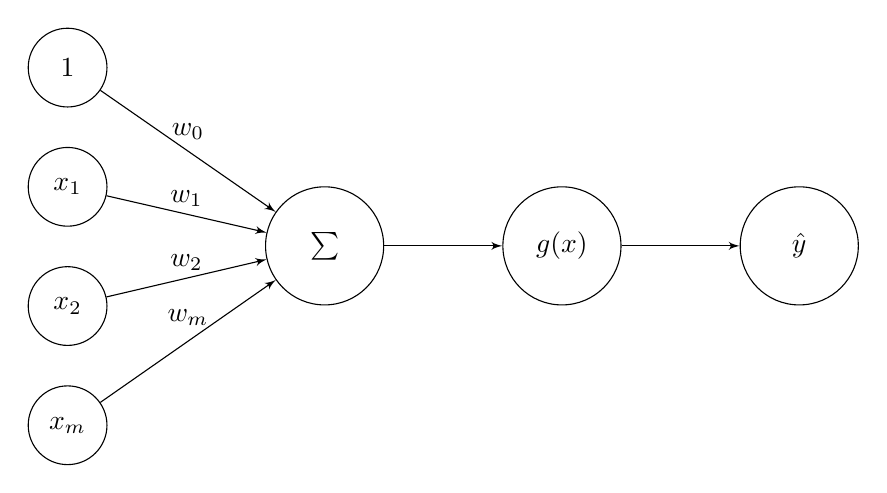
\begin{tikzpicture} [>=latex', node distance = 2cm]
            % Set primary nodes
            \tikzset{
                entity/.style={
                        rectangle,
                        draw
                    }
            }
            \tikzset{
                inputNode/.style={
                        draw,
                        circle,
                        minimum height=1cm
                    }
            }
            \tikzset{
                sumNode/.style={
                        draw,
                        circle,
                        minimum height=1.5cm
                    }
            }
            \tikzset{
                activationNode/.style={
                        draw,
                        circle,
                        minimum height=1.5cm
                    }
            }
            \tikzset{
                outNode/.style={
                        draw,
                        circle,
                        minimum height=1.5cm
                    }
            }
            % Placing nodes
            \node[inputNode](bias){$1$};
            \node[inputNode, below = 0.5cm of bias](x1){$x_1$};
            \node[inputNode, below = 0.5cm of x1](x2){$x_2$};
            \node[inputNode, below = 0.5cm of x2](xm){$x_m$};
            \node[sumNode, right = 2cm of x1, yshift = -0.75cm](sum){$\sum$};
            \node[activationNode, right = 1.5cm of sum](gx){$g(x)$};
            \node[outNode, right = 1.5cm of gx](out){$\hat y$};
            % Placing arrows
            \draw[->](bias) edge node[yshift = 0.25cm]{$w_0$} (sum);
            \draw[->](x1) edge node[yshift = 0.2cm]{$w_1$} (sum);
            \draw[->](x2) edge node[yshift = 0.2cm]{$w_2$} (sum);
            \draw[->](xm) edge node[yshift = 0.3cm]{$w_m$} (sum);
            \draw[->](sum) edge (gx);
            \draw[->](gx) edge (out);
        \end{tikzpicture}
    \end{center}
    \caption{Model of perceptron}
\end{figure}
\begin{equation}
    \hat y = g \Bigg( w_0 + \sum_{i=1}^{m}x_i w_i \Bigg)
\end{equation}
With:
\begin{conditions}
    g & Activation function \\
    w_o & Bias
\end{conditions}
In vector form:
\begin{equation}
    \hat y = g(W_0 + X^TW)
\end{equation}
With:
\begin{conditions}
    W & $\begin{pmatrix} w_1 \\ \vdots \\ w_m \end{pmatrix}$ , X = $\begin{pmatrix} x_1 \\ \vdots \\ x_m \end{pmatrix}$
\end{conditions}
As seen, in a conventional model of a perceptron every input of an
layer is multiplied by a weighting. It can be seen, that the implementation
of such a perceptron can be handled by given hardware architecture like GPU's
or matrix multiplier, because of the possibility to proceed every input matrix
and their associated weight matrix independently.

\subsection{Activation function}
The activation function of a perceptron has the purpose to determines the
behavior of the perceptron in response to external stimuli. There are different
kinds of activation functions which can be used for different purpuse.

\pagebreak
\section{Design Overview}
The hardware of this project consist of a 32-bit microcontroller named SAM D21/DA1 and a
Cyclone 10 FPGA. Both chips are placed on a board, so called Arduino Vidor 4000. This board
comes with an USB interface, which will be the communication between frontend (PC) and
the executing hardware. The figure \ref{fig:abstractHardwareDescription} show the most
abstract hardware model. This model show the mentioned frontend and hardware, but also the
"Top Level Resolver", which distribute the data to either the storage, which holds the data to
be proceed, or the new settings for the single perceptron activation functions. In the concret
model, the address line has a size of 11-Bit and the data line a size of 4-Bit. This results
in a maximum count of 256 perceptrons in 16 layers, if one perceptron of the incomming layer
is connected with all perceptrons of the previous outgoing layer. The load line tell the single
perceptrons, that they can storage the new information after addressing. The address line needs to be a
11-Bit one, causing the fact, that every oerceptron needs 5 informations to store. More related to this
will be described later. For simlifity purpose, the clock and reset signals for every single module
is not shown in the figure.

% Top Level Hardware Model Diagram
\begin{figure}[htbp]
    \begin{center}
        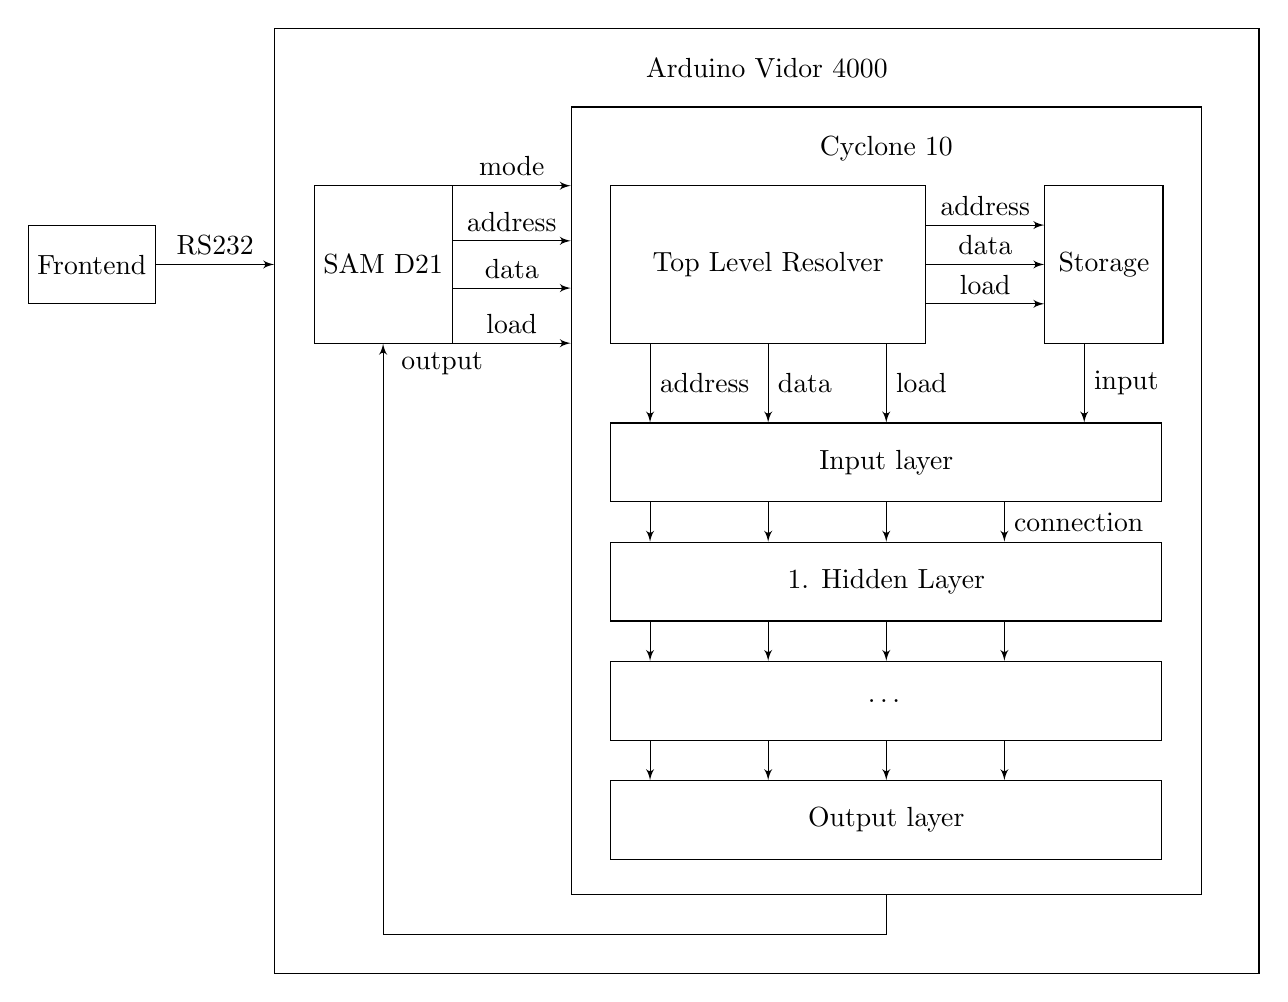
\begin{tikzpicture} [>=latex', node distance = 2cm]
            % Set primary nodes
            \tikzset{
                entity/.style={
                        rectangle,
                        draw
                    }
            }
            \tikzset{
                frontendNode/.style={
                        draw,
                        rectangle,
                        minimum height=1cm,
                        minimum width=1.5cm,
                    }
            }
            \tikzset{
                samd21Node/.style={
                        draw,
                        rectangle,
                        minimum height=2cm,
                        minimum width=1.5cm,
                    }
            }
            \tikzset{
                vidorNode/.style={
                        draw,
                        rectangle,
                        minimum height=12cm,
                        minimum width=12.5cm,
                        text depth = 11cm
                    }
            }
            \tikzset{
                fpgaNode/.style={
                        draw,
                        rectangle,
                        minimum height=10cm,
                        minimum width=8cm,
                        text depth = 9cm
                    }
            }
            \tikzset{
                resolverNode/.style={
                        draw,
                        rectangle,
                        minimum height=2cm,
                        minimum width=4cm
                    }
            }
            \tikzset{
                storageNode/.style={
                        draw,
                        rectangle,
                        minimum height=2cm,
                        minimum width=1.5cm
                    }
            }
            \tikzset{
                layerNode/.style={
                        draw,
                        rectangle,
                        minimum height=1cm,
                        minimum width=7cm
                    }
            }
            \tikzset{
                arrow/.style={
                        thick,
                        ->,
                        >=sealth
                    }
            }
            % Configure arrows
            \tikzstyle{arrow} = [thick, ->, >=stealth]
            % Placing nodes
            \node[frontendNode](frontend){Frontend};
            \node[vidorNode, right = 1.5cm of frontend, yshift = -3cm](vidor){Arduino Vidor 4000};
            \node[samd21Node, right = 2cm of frontend](samd21){SAM D21};
            \node[fpgaNode, right = 1.5cm of samd21, yshift = -3cm](fpga){Cyclone 10};
            \node[resolverNode, right = 2cm of samd21](resolver){Top Level Resolver};
            \node[storageNode, right = 1.5cm of resolver](storage){Storage};
            \node[layerNode, below = 1cm of resolver, xshift = 1.5cm](input){Input layer};
            \node[layerNode, below = 0.5cm of input](hidden1){1. Hidden Layer};
            \node[layerNode, below = 0.5cm of hidden1](hidden2){\dots};
            \node[layerNode, below = 0.5cm of hidden2](output){Output layer};
            % Draw arrows
            \draw[->](frontend.east) -- ++(1.5,0) node[midway,above]{RS232};
            \draw[->](samd21.east) ++(0,1) -- ++(1.5,0) node[midway,above]{mode};
            \draw[->](samd21.east) ++(0,0.3) -- ++(1.5,0) node[midway,above]{address};
            \draw[->](samd21.east) ++(0,-0.3) -- ++(1.5,0) node[midway,above]{data};
            \draw[->](samd21.east) ++(0,-1) -- ++(1.5,0) node[midway,above]{load};
            \draw[->](resolver.east) ++(0,0.5) -- ++(1.5,0) node[midway,above]{address};
            \draw[->](resolver.east) ++(0,0) -- ++(1.5,0) node[midway,above]{data};
            \draw[->](resolver.east) ++(0,-0.5) -- ++(1.5,0) node[midway,above]{load};
            \draw[->](resolver.south) ++(-1.5,0) -- ++(0,-1) node[midway,sloped,right, rotate=90]{address};
            \draw[->](resolver.south) ++(0,0) -- ++(0,-1) node[midway,sloped,right, rotate=90]{data};
            \draw[->](resolver.south) ++(1.5,0) -- ++(0,-1) node[midway,sloped,right, rotate=90]{load};
            \draw[->](storage.south) ++(-0.25,0) -- ++(0,-1) node[midway,sloped,right, rotate=90]{input};
            \draw[->](input.south) ++(-3,0) -- ++(0,-0.5);
            \draw[->](input.south) ++(-1.5,0) -- ++(0,-0.5);
            \draw[->](input.south) ++(0,0) -- ++(0,-0.5);
            \draw[->](input.south) ++(1.5,0) -- ++(0,-0.5) node[midway,sloped,right, rotate=90]{connection};
            \draw[->](hidden1.south) ++(-3,0) -- ++(0,-0.5);
            \draw[->](hidden1.south) ++(-1.5,0) -- ++(0,-0.5);
            \draw[->](hidden1.south) ++(0,0) -- ++(0,-0.5);
            \draw[->](hidden1.south) ++(1.5,0) -- ++(0,-0.5);
            \draw[->](hidden2.south) ++(-3,0) -- ++(0,-0.5);
            \draw[->](hidden2.south) ++(-1.5,0) -- ++(0,-0.5);
            \draw[->](hidden2.south) ++(0,0) -- ++(0,-0.5);
            \draw[->](hidden2.south) ++(1.5,0) -- ++(0,-0.5);
            \draw[->](fpga.south) -- ++(0,-0.5) -| (samd21.south);
            \draw (samd21.south) ++(0.75,-0.25) node[]{output};
        \end{tikzpicture}
        \caption{Top Level Hardware Model}
        \label{fig:abstractHardwareDescription}
    \end{center}
\end{figure}\pagebreak

Every layer of the hardware model consists of a "Layer Resolver", which takes care about the
signal distribution to every single perceptron. This has the advantage, that the data lines
inside the single layer model can be recduced. In the concrete hardware model, the 11-Bit
address line go through all the layer resolvers, which split them in a 7-Bit address line, which
is connected to every perceptron in the particular layer. The data line stay a 4-Bit and the load
line a 1-Bit connection and are simply y-splitted in the resolver.
% Layer Level Hardware Model Diagram
\begin{figure}[htbp]
    \begin{center}
        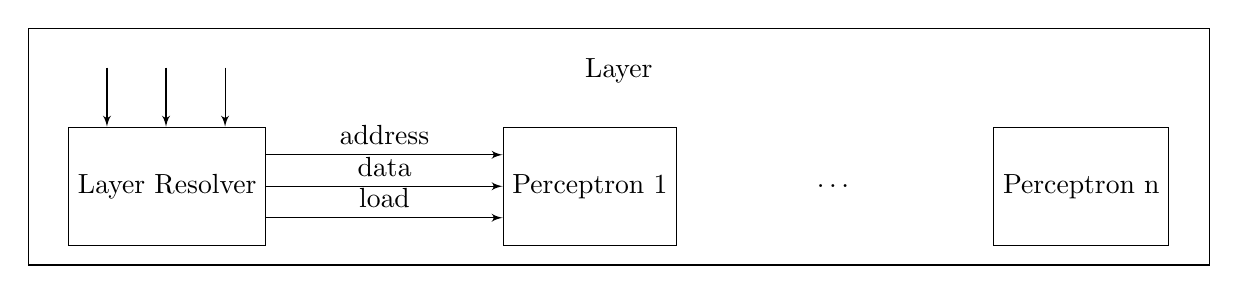
\begin{tikzpicture} [>=latex', node distance = 2cm]
            % Set primary nodes
            \tikzset{
                entity/.style={
                        rectangle,
                        draw
                    }
            }
            \tikzset{
                layerNode/.style={
                        draw,
                        rectangle,
                        minimum height=3cm,
                        minimum width=15cm,
                        text depth = 2cm
                    }
            }
            \tikzset{
                layerResolverNode/.style={
                        draw,
                        rectangle,
                        minimum height=1.5cm,
                        minimum width=2.5cm,
                    }
            }
            \tikzset{
                perceptronNode/.style={
                        draw,
                        rectangle,
                        minimum height=1.5cm,
                        minimum width=2cm,
                    }
            }
            % Configure arrows
            \tikzstyle{arrow} = [thick, ->, >=stealth]
            % Placing nodes
            \node[layerNode](layer){Layer};
            \node[layerResolverNode, right = 0cm of layer, xshift = -14.5cm, yshift = -0.5cm](layerResolver){Layer Resolver};
            \node[perceptronNode, right = 3cm of layerResolver](perceptron1){Perceptron 1};
            \node[perceptronNode, right = 1cm of perceptron1, draw=none](perceptron2){\dots};
            \node[perceptronNode, right = 1cm of perceptron2](perceptron3){Perceptron n};
            % Draw arrows
            \draw[->](layer.north) ++(-6.5,-0.5) -- ++(0,-0.75);
            \draw[->](layer.north) ++(-5.75,-0.5) -- ++(0,-0.75);
            \draw[->](layer.north) ++(-5,-0.5) -- ++(0,-0.75);
            \draw[->](layerResolver.east) ++(0,0.4) -- ++(3,0) node[midway,sloped,yshift=0.25cm]{address};
            \draw[->](layerResolver.east) ++(0,0) -- ++(3,0) node[midway,sloped,yshift=0.25cm]{data};
            \draw[->](layerResolver.east) ++(0,-0.4) -- ++(3,0) node[midway,sloped,yshift=0.25cm]{load};

        \end{tikzpicture}
        \caption{Layer Level Hardware Model}
        \label{fig:layerHardwareModel}
    \end{center}
\end{figure}
\FloatBarrier

The perceptron itselfe consist of a two state input control instead of float point calculations. That
means, that the connection from one perceptron output to an other perceptron input can only be active
or non active. Furthermore, the second parameter inside the perceptron is the activation function, which
is basically the summation over a count of input "high" signals. If the summation is greater than a given
value, the output of the perceptron is pulled "high".

\section{Implementation}
The implemetation of the whole system is based on the hardware overview and splitted in different modules
which finally get connected with each other.

\section{Validation}


\end{document}